\documentclass[a4paper,12pt,gray]{article}

\usepackage{préambule}

\TitreDActivite{Activité : Promenades sur une droite}

\definecolor{block1}{RGB}{230, 230, 230}
\definecolor{block2}{RGB}{180, 180, 180}

\newcommand{\blockHeight}{0.9}
\newcommand{\blockWidth}{5}
\newcommand{\clipPosition}{1}
\newcommand{\clipHeight}{0.16}

\newcounter{codeBlockCounter}
\newcounter{codeBlockCounterBinary}
\setcounter{codeBlockCounter}{0}
\setcounter{codeBlockCounterBinary}{0}

\newcommand{\instruction}[1]{
	\coordinate (BlockStart) at (0,-\thecodeBlockCounter*\blockHeight);
	\ifthenelse{\equal{\thecodeBlockCounterBinary}{0}}{
		\addtocounter{codeBlockCounterBinary}{1}
		\draw[fill=block1] (BlockStart)
			-- ++(\clipPosition,0)
			-- ++(\clipHeight,-\clipHeight)
			-- ++(\clipHeight/2,0)
			-- ++(\clipHeight,\clipHeight)
			-- ++(\blockWidth-\clipPosition-2.5*\clipHeight,0)
			-- ++(0,-\blockHeight)
			-- ++(-\blockWidth+\clipPosition+2.5*\clipHeight,0)
			-- ++(-\clipHeight,-\clipHeight)
			-- ++(-\clipHeight/2,0)
			-- ++(-\clipHeight,\clipHeight)
			-- ++(-\clipPosition,0)
			-- ++(0,\blockHeight);
	}{
		\addtocounter{codeBlockCounterBinary}{-1}
		\draw[fill=block2] (BlockStart)
			-- ++(\clipPosition,0)
			-- ++(\clipHeight,-\clipHeight)
			-- ++(\clipHeight/2,0)
			-- ++(\clipHeight,\clipHeight)
			-- ++(\blockWidth-\clipPosition-2.5*\clipHeight,0)
			-- ++(0,-\blockHeight)
			-- ++(-\blockWidth+\clipPosition+2.5*\clipHeight,0)
			-- ++(-\clipHeight,-\clipHeight)
			-- ++(-\clipHeight/2,0)
			-- ++(-\clipHeight,\clipHeight)
			-- ++(-\clipPosition,0)
			-- ++(0,\blockHeight);
	}
	\node[anchor=west] at (0.5,-\thecodeBlockCounter*\blockHeight - \blockHeight/2) {#1};
	\addtocounter{codeBlockCounter}{1}
}

\begin{document}

\maketitle

\begin{center}
	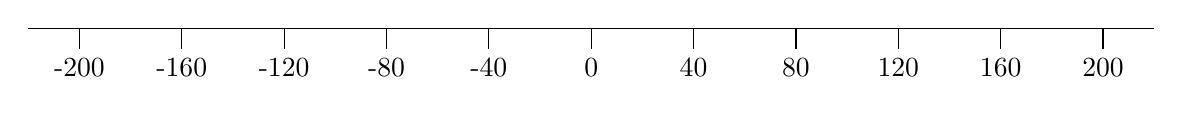
\begin{tikzpicture}[scale=1.3]
		\draw[\myArrow] (-5.5,0) -- (5.5,0);
		\foreach \pos/\x in {
				-200/-5,
				-160/-4,
				-120/-3,
				-80/-2,
				-40/-1,
				0/0,
				40/1,
				80/2,
				120/3,
				160/4,
				200/5,
			} {
				\draw (\x,0) -- ++(0,-0.2) node[below] {\pos};
			}
	\end{tikzpicture}
\end{center}

\begin{exercice}\

	On déplace un personnage sur une droite. Pour se déplacer, celui-ci suit une série d'instructions.

	\vspace{1em}

	\begin{center}
		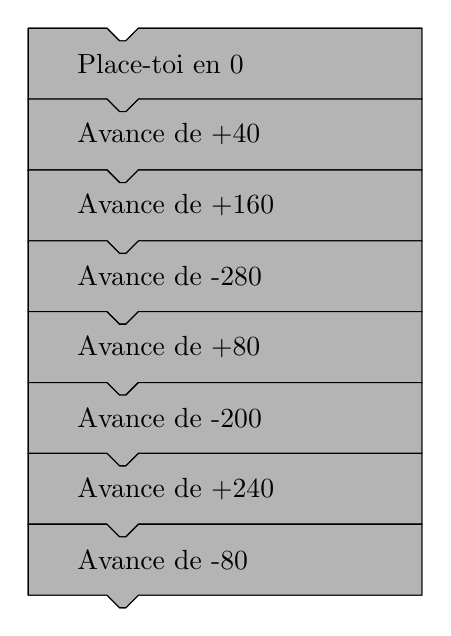
\begin{tikzpicture}
			\instruction{Place-toi en \squared{0}}
			\instruction{Avance de \squared{+40}}
			\instruction{Avance de \squared{+160}}
			\instruction{Avance de \squared{-280}}
			\instruction{Avance de \squared{+80}}
			\instruction{Avance de \squared{-200}}
			\instruction{Avance de \squared{+240}}
			\instruction{Avance de \squared{-80}}
		\end{tikzpicture}
	\end{center}

	\begin{enumerate}
		\item Où arrive le personnage si il suit ces instructions ? ........
		\item Si on enlève le block “Avance de \squared{40}”, où arrive le personnage ? ........
		\item On remet le block précédent, et on enlève cette fois le block “Avance de \squared{-200}”. Où arrive le personnage ? ........
	\end{enumerate}
\end{exercice}

\end{document}